\documentclass[MASTER.tex]{subfiles} 
\begin{document} 
%===========================================================
\begin{frame}
Important Components of the Python Scientific Stack
\end{frame}
%===========================================================%
\begin{frame}
\frametitle{Continuum Analytics’ Anaconda}
Anaconda, a free product of Continuum Analytics (www.continuum.io), is a virtually complete scientific
stack for Python. It includes both the core Python interpreter and standard libraries as well as most
modules required for data analysis. Anaconda is free to use and modules for accelerating the performance
of linear algebra on Intel processors using the Math Kernel Library (MKL) are available (free to
academic users and for a small cost to non-academic users). 
\end{frame}
%===========================================================%
\begin{frame}
Continuum Analytics also provides other
high-performance modules for reading large data files or using theGPUto further accelerate performance
for an additional, modest charge. 
\end{frame}
%===========================================================%
\begin{frame}
\frametitle{Installing Anaconda}
Most importantly, installation is extraordinarily easy onWindows, Linux
and OS X. Anaconda is also simple to update to the latest version using
conda update conda
conda update anaconda
\end{frame}
%===========================================================%
\begin{frame}
\frametitle{NumPy}
NumPy provides a set of array and matrix data types which are essential for statistics, econometrics and
data analysis.
\end{frame}
%===========================================================%
\begin{frame}
\frametitle{SciPy}
SciPy contains a large number of routines needed for analysis of data. 

The most important include a wide
range of random number generators, linear algebra routines and optimizers. 

SciPy depends on NumPy.
\end{frame}
%===========================================================%
\begin{frame}
\frametitle{IPython}
IPython provides an interactive Python environment which enhances productivity when developing code
or performing interactive data analysis.
\end{frame}
%===========================================================%
\begin{frame}
	
	\begin{figure}
\centering
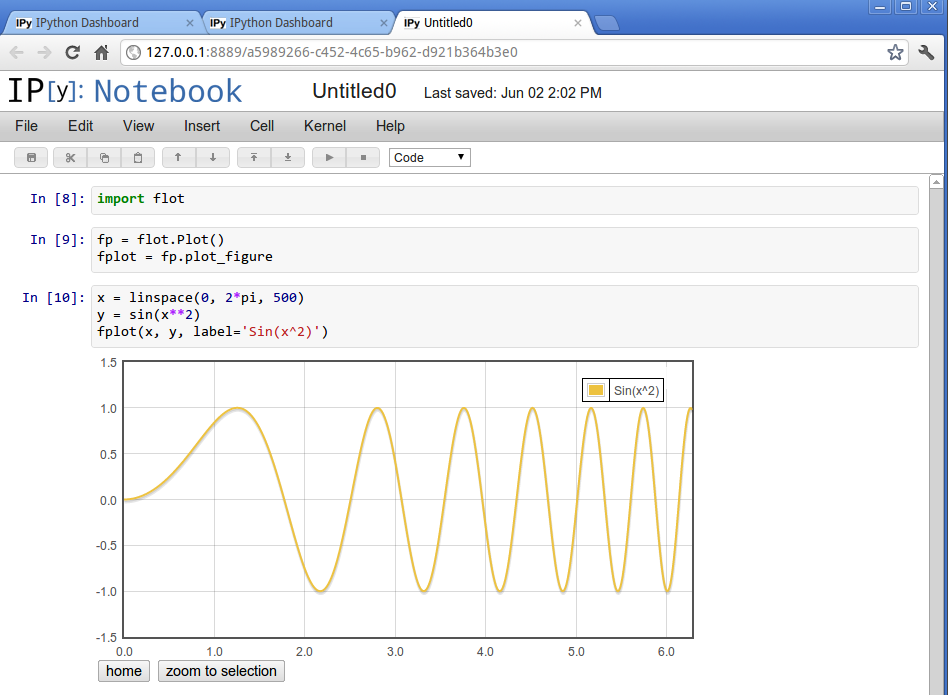
\includegraphics[width=0.9\linewidth]{vk2Q6}

\end{figure}

\end{frame}
%===========================================================%

\begin{frame}
	
	\begin{figure}
\centering

\includegraphics[width=0.7\linewidth]{jupyter}
\caption{}
\label{fig:jupyter}
\end{figure}

\end{frame}
	
%===========================================================%
\begin{frame}
\frametitle{matplotlib and seaborn}
\large
\begin{itemize}
\item matplotlib provides a plotting environment for 2D plots, with limited support for 3D plotting. 
\item seaborn is
a Python package that improves the default appearance of matplotlib plots without any additional code.
\end{itemize}

\end{frame}
%===========================================================%
\begin{frame}
	\frametitle{PyData :  Conference Mission}
\large
	

PyData is a gathering of users and developers of data analysis tools in Python. The goals are to provide Python enthusiasts a place to share ideas and learn from each other about how best to apply our language and tools to ever-evolving challenges in the vast realm of data management, processing, analytics, and visualization.

\end{frame}
%===========================================================%
\begin{frame}
\large
\frametitle{PyData}
\begin{itemize}
\item We aim to be an accessible, community-driven conference, with tutorials for novices, advanced topical workshops for practitioners, and opportunities for package developers and users to meet in person.

\item A major goal of the conference is to provide a venue for users across all the various domains of data analysis to share their experiences and their techniques, as well as highlight the triumphs and potential pitfalls of using Python for certain kinds of problems.
\end{itemize}
\end{frame}
%===========================================================%
\begin{frame}
\frametitle{pandas}
\begin{itemize}
\item pandas provides high-performance data structures.
\end{itemize}
\end{frame}
%===========================================================%
\begin{frame}
	\frametitle{pandas}
	\textit{pandas} is a high-performance module that provides a comprehensive set of structures for working with
	data. \textit{pandas} excels at handling structured data, such as data sets containing many variables, working with
	missing values and merging across multiple data sets. 
\end{frame}
%===========================================================%
\begin{frame}
	\large
	\frametitle{pandas}	
	\begin{itemize}
	
	\item While extremely useful, \textit{pandas} is not an essential component of the Python scientific stack unlike NumPy, SciPy or matplotlib, and so while \textit{pandas} doesn’t
	make data analysis possible in Python, it makes it much easier. \item \textit{pandas} also provides high-performance,
	robust methods for importing from and exporting to a wide range of formats.
	\end{itemize}
\end{frame}
%===========================================================%
\begin{frame}
	
	\large
\frametitle{Performance Modules : Cython and Numba}
A number of modules are available to help with performance. These include Cython and Numba.

\begin{description}
	\item[Cython] Cython
	is a Python module which facilitates using a simple Python-derived creole to write functions that can be
	compiled to native (C code) Python extensions. 
	
	
	\item[Numba] 
	Numba uses a method of just-in-time compilation to
	translate a subset of Python to native code using \textit{Low-Level Virtual Machine} (LLVM).
\end{description} 

\end{frame}
%=======================================================================%
\end{document}